%%% -*- mode:latex; mode:flyspell -*-

%%% Local Variables:
%%% TeX-master: "mu2e-36575"
%%% End:
\section{Tuning the calorimeter timing resolution}

The calorimeter timing simulation has been significantly improved since the Offline version
v9\_0\_5 used to start SU2020 branch.
The old timing simulation was largely underestimating the calorimeter timing resolution.
A better parametrization of the photon propagation time inside the crystal and, most significantly, a better implementation of the noise in the simulation in more recent versions of the Offline produces  simulation results much closer to the test beam measurements \cite{MU2E_35540_CALO_TIMING}.

The different components of the calorimeter noise during the first period of data taking have been estimated in \cite{MU2E_35519_CALO_NOISE} 
assuming the Run Plan reported in \cite{MU2E_33731_RUN1_PLAN}, where the results are summarized
in Table \ref{table:calonoise}. 
The noise components include the electronic noise (measured at the cosmic ray stand), 
radiation induced noise (RIN), and dark current due to neutron radiation damage
in the SiPMs (assuming an operation temperature of $-10^o$ C).
A safety factor of 2 has been used for the  neutron induced noise to reflect the uncertainty of the results of neutron radiation damage measurements.

\begin{table}[htbp]
  \begin{center} 
    \begin{tabular}{|c|c|c|c|c|}
      \hline
      Run 1 period      & FEE noise  & RIN     & Dark current noise & RIN$\oplus$Dark    \\ 
      \hline
      1 batch start     & 200 keV    & 280 keV &  --                & 344 keV  \\
      1 batch end       & 200 keV    & 280 keV &  450 keV           & 566 keV  \\
      2 batch end       & 200 keV    & 400 keV &  492 keV           & 634 keV  \\
      \hline
    \end{tabular}
  \end{center}
  \caption{
  \label{table:calonoise}
    Calorimeter noise levels in different Run 1 periods as estimated in \cite{MU2E_35519_CALO_NOISE}. 
  }
  % \vspace{0.5in}
\end{table}

Using the results in the Table \ref{table:calonoise}, we assume an average noise of 455 keV
for the 1 batch period and 600 keV for the 2 batch period. 
A parametrization of the time resolution as function of the RIN$\oplus$Dark noise level (assuming FEE noise fixed at 200 keV) and the energy deposited
in a crystal obtained using the latest calorimeter simulation software has been presented in  \cite{MU2E_36225_CALO_TIME_RES}.
The curves corresponding to a RIN$\oplus$Dark noise of 455 keV and 600 keV are the lower dashed
lines in Figures \ref{fig:calorimeter_timing_resolution_1batch} and  \ref{fig:calorimeter_timing_resolution_2batch}.

Table \ref{table:calonoise} does not include the time jitter of the accelerator signal.
This effect should also be included in the tracker timing simulation, where it is currently
ignored. For particle identification, the only relevant quantity is the relative time
between the tracker and calorimeter. 
We decided not to change the tracker timing simulation, but instead to add the accelerator
clock jitter only to the cluster time.
Preliminary measurements \cite{MU2E_35392_TIME_JITTER} show a time jitter of 172 ps
for a chain of 2 DTCs and 217 ps for a chain of 7 DTCs. We take 200 ps as our best estimate.

Integration of the latest updates to the calorimeter simulation software into the SU2020 branch
would be a task, very complicated technically. Instead, an additional Gaussian time smearing
component is added to the  CaloCrystalHitFromHit module to reproduce the desired time resolution. 

Figures \ref{fig:calorimeter_timing_resolution_1batch} and  \ref{fig:calorimeter_timing_resolution_2batch} show the output of the time resolution
simulation with the additional Gaussian smearing component as a function of the energy deposited
in the crystal for the two calorimeter disks for 1 and 2 batch modes.
The agreement with the expected analytical function is shown. 
The deviations at small energies are not important as the time resolution simulation
in those regions is known to be less reliable.

\begin{figure}[h]
%  \hspace{-0.6in}
  \begin{tikzpicture}
    \node[anchor=south west,inner sep=0] at (0.,0.) {
      % \node[shift={(0 cm,0.cm)},inner sep=0,rotate={90}] at (0,0) {}
      \makebox[\textwidth][c] {
        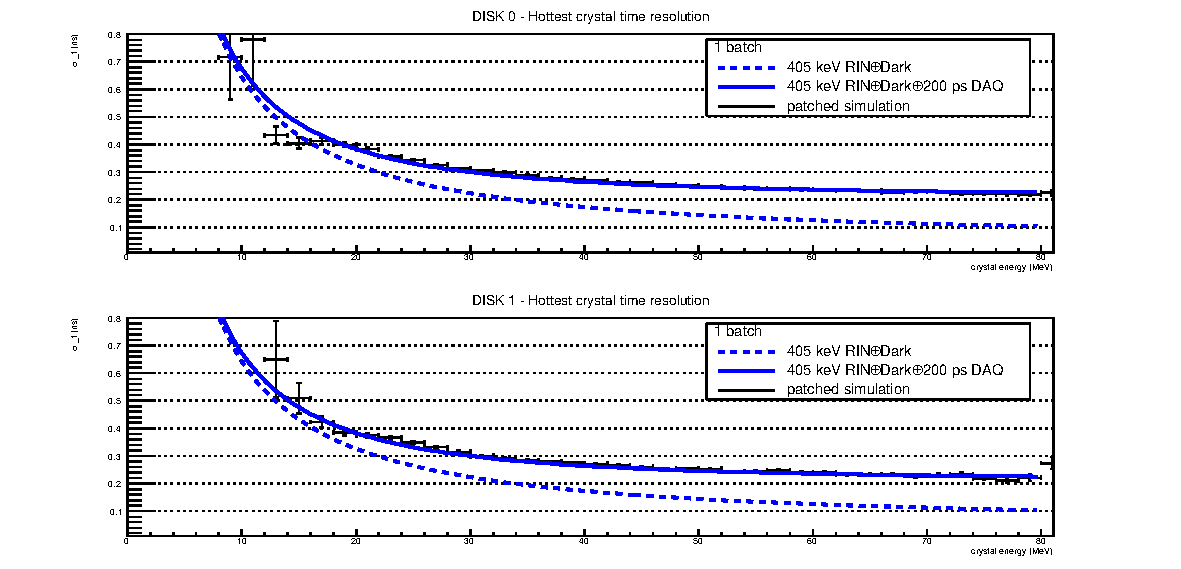
\includegraphics[width=0.90\textwidth, trim = 40 0 125 0, clip]{figures/pdf/figure_00401_sigmat_1batch_corrected}
      }
    };
    % \node [text width=6cm, scale=0.8] at (4.5,6.4) {mu2e-18894 by Kevin Lynch and Jim Popp};
  \end{tikzpicture}
  % \captionof{figure} {
  \caption{
    \label{fig:calorimeter_timing_resolution_1batch}
    Tuning of the calorimeter timing resolution for the 1 batch run period.
    The lower dashed curve corresponds to the parametrization given in 
    \cite{MU2E_36225_CALO_TIME_RES} using a noise of 455 keV.
    The upper dashed curve includes the 200 ps for the DTCs time jitter.
    The black points represent the results of the SU2020 patched calorimeter time simulation.
  }
\end{figure}

\begin{figure}[h]
%  \hspace{-0.6in}
  \begin{tikzpicture}
    \node[anchor=south west,inner sep=0] at (0.,0.) {
      % \node[shift={(0 cm,0.cm)},inner sep=0,rotate={90}] at (0,0) {}
      \makebox[\textwidth][c] {
        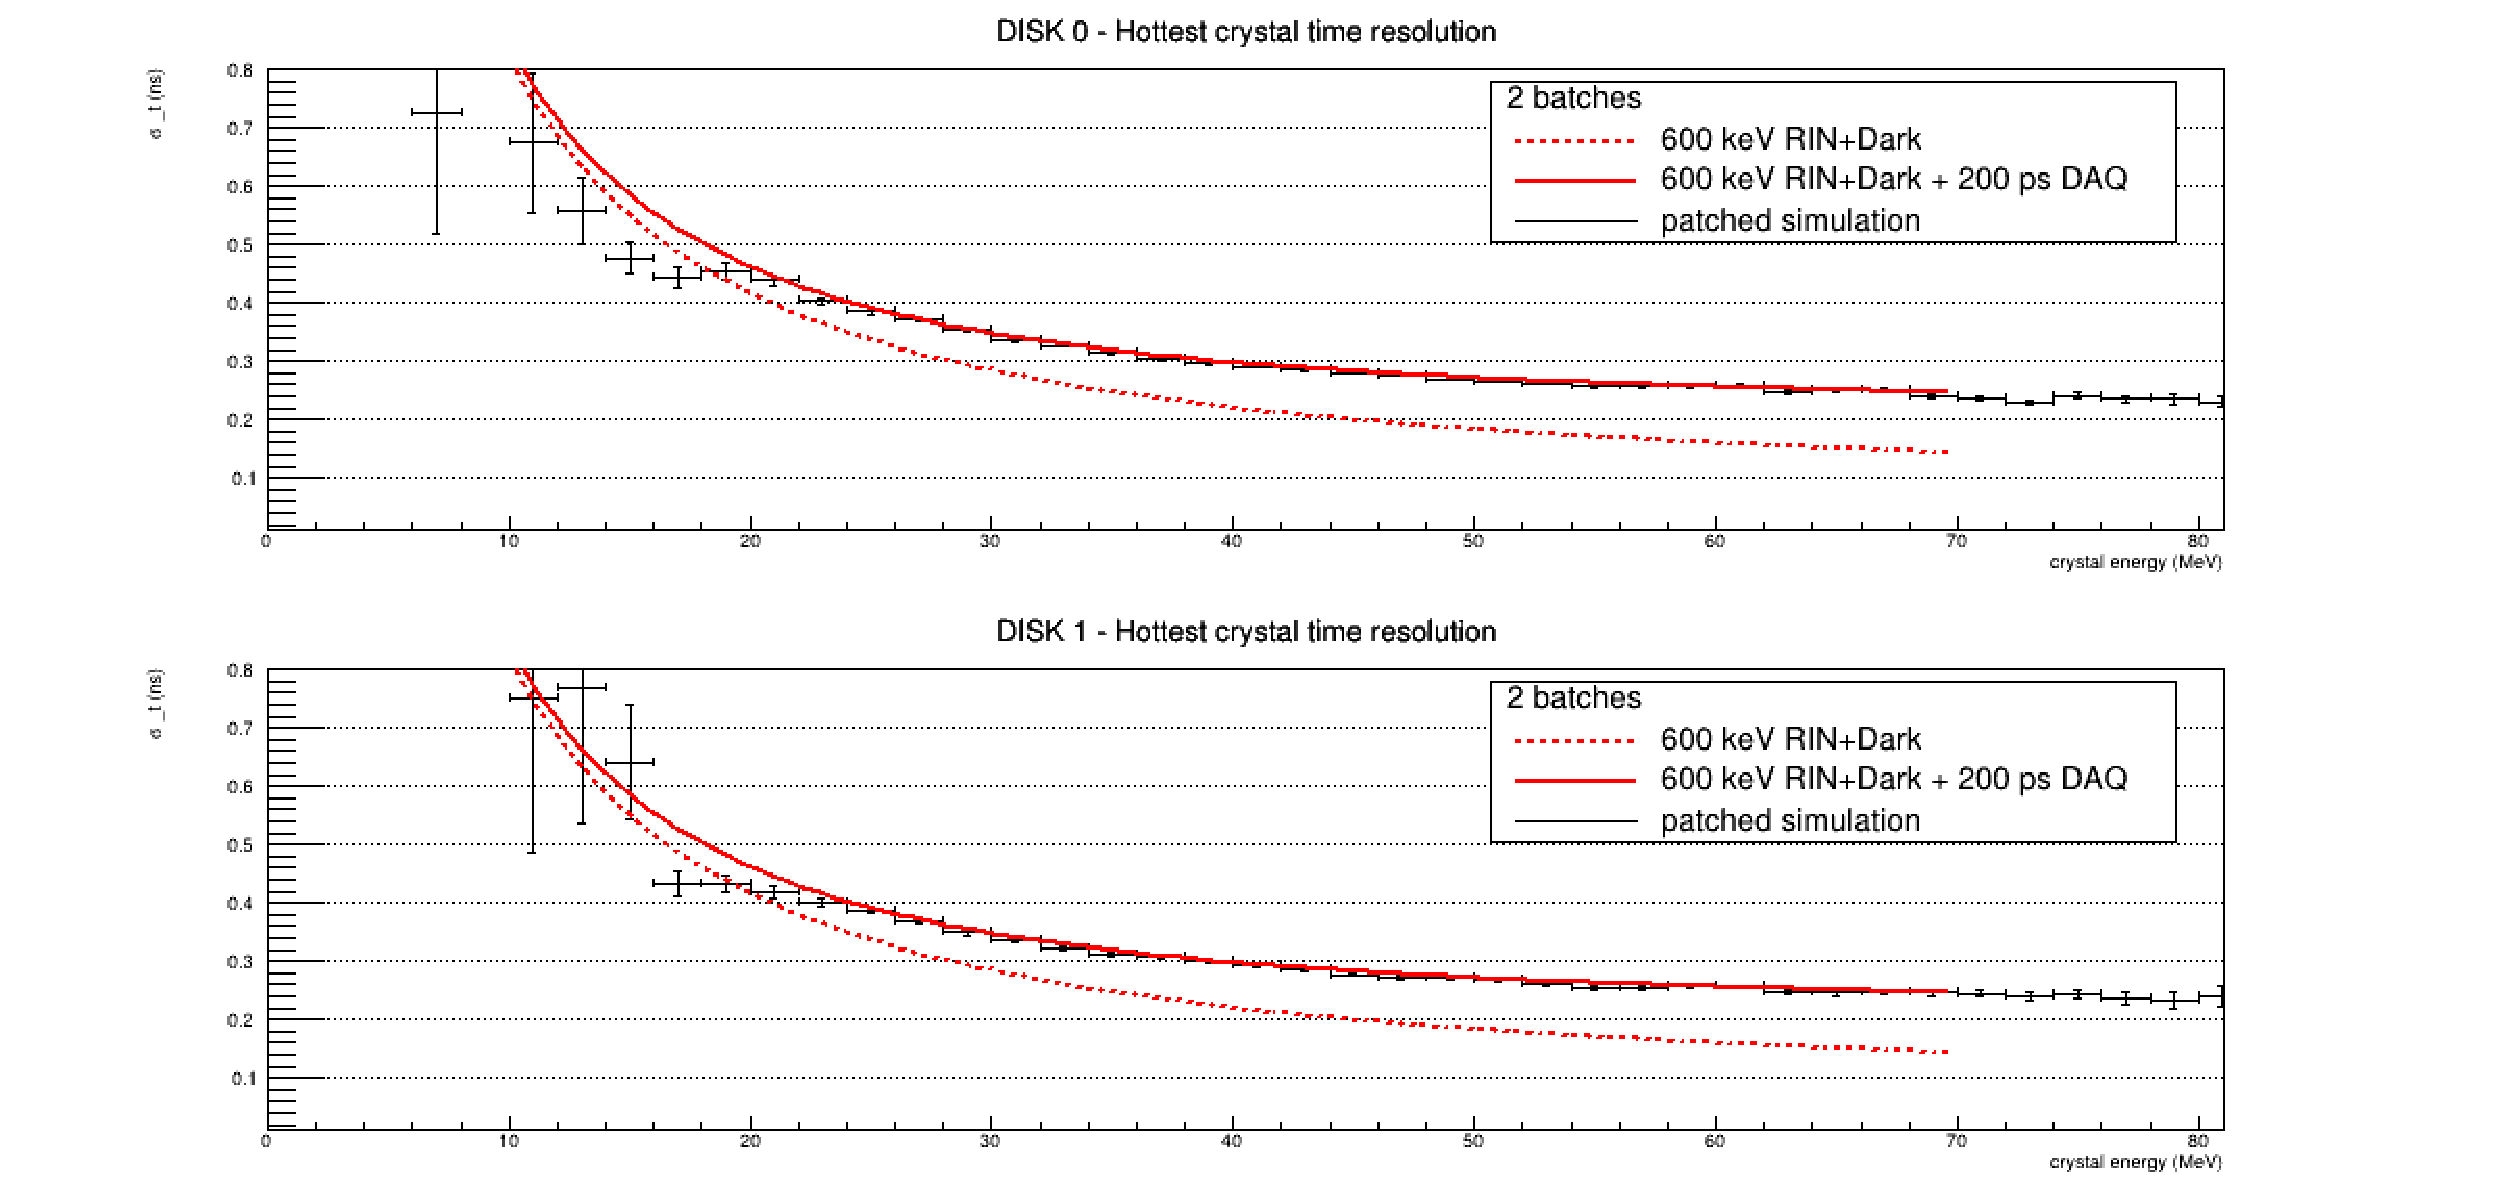
\includegraphics[width=0.90\textwidth, trim = 40 0 125 0, clip]{figures/pdf/figure_00402_sigmat_2batch_corrected}
      }
    };
    % \node [text width=6cm, scale=0.8] at (4.5,6.4) {mu2e-18894 by Kevin Lynch and Jim Popp};
  \end{tikzpicture}
  % \captionof{figure} {
  \caption{
    \label{fig:calorimeter_timing_resolution_2batch}
    Tuning of the calorimeter timing resolution for the 2 batch run period.
    The lower dashed curve corresponds to the parametrization
    given in \cite{MU2E_36225_CALO_TIME_RES} using a noise of 600 keV.
    The upper dashed curve includes the 200 ps for the DTCs time jitter.
    The black points represent the results of the SU2020 patched calorimeter time simulation. 
  }
\end{figure}
